\documentclass{article}

\usepackage{titlesec}
\usepackage{amsmath}
\usepackage{amsfonts}
\usepackage{graphicx}
\usepackage{float}
\title{Numerical Methods for Ordinary Differential Equations}
\author{Murray Heymann \\
	Technische Universit{\"a}t Kaiserslautern \\
	413121}
\date{\today}


\titleformat{\section}{\normalfont \LARGE \bfseries}
{Problem\ Sheet\ \thesection}{2.3ex plus .2ex}{}
\titleformat{\subsection}{\normalfont \Large \bfseries}
{Question\ \thesubsection}{2.3ex plus .2ex}{}
\titlespacing{\subsubsection}{2em}{*1}{*1}

\begin{document}
\maketitle


\section{}
\subsection{}
\begin{itemize}
	\item[(a)]
		The solution to the differential equation is \[ x(t) = e
		^{- \lambda t} x_0.\]

		The explicit equation for calculating $x_{j + 1}$ reads
		\begin{align*}
			x_{j + 1} &= x_j + \tau (-\lambda) x_j \\
			&= (1 - \tau \lambda) x_j \\
			&= (1 - \tau \lambda)^{j+1} x_0 \\
			&= (1 - \tau \lambda)^{j+1},
		\end{align*} where $\tau$ is the the time interval between time
		sample points.
		Notice that for all values of $\lambda$, $e^{-\lambda t}$
		converges to $0$ as $t$ gets large.  However, if we choose
		$\tau$ and $\lambda$ such that $\tau \lambda > 2$, our recursive
		equation for $x_{j+1}$ describes a divergent sequence of
		numbers. It is therefore important to choose appropriately small
		values for $\tau$.

		We draw the graph for various values of $\lambda$.
		\begin{figure}[H]
			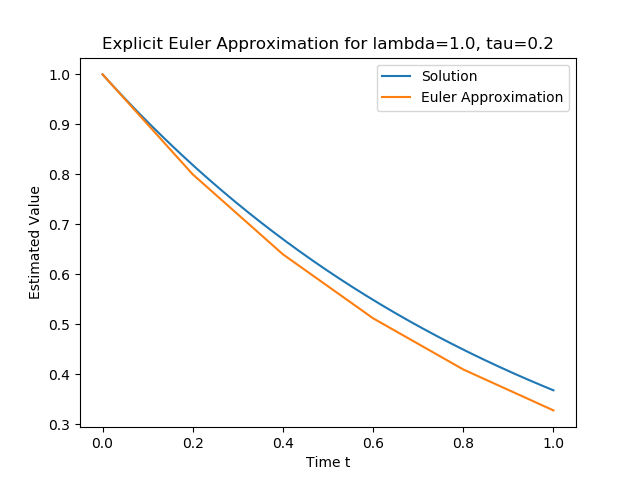
\includegraphics[scale=0.6]{graph1a_1_02}
		\end{figure}

		For too large $\lambda \tau$, we see the divergent behaviour:
		\begin{figure}[H]
			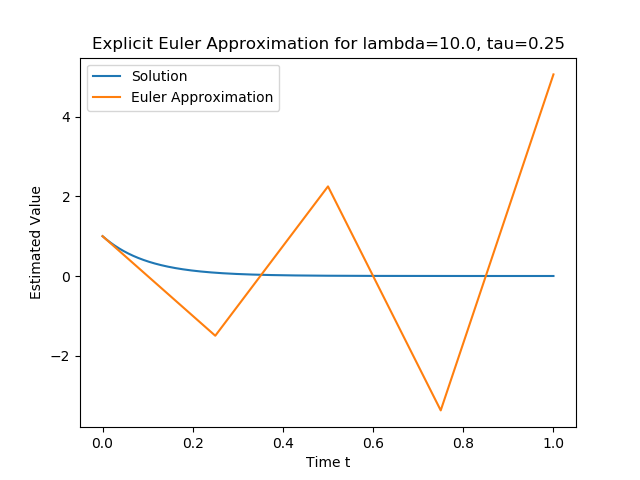
\includegraphics[scale=0.6]{graph1a_10_025}
		\end{figure}

		We consider the local order analytically.  To calculate this, we
		consider the
		error after a single iteration, that is $\epsilon(\tau) =
		|e^{-\lambda \tau} - x_1|$.  We work under the assumption that
		$\tau \in (0,1]$.  Notice
		\begin{align*}
			e^{- \lambda} &= \sum_{k=0}^{\infty}
			\frac{(-1)^k(\lambda^k)}{k!} \\
			e^{- \lambda} &= 1 - \lambda + \frac{\lambda^2}{2}
			- \frac{\lambda^3}{3!} \ldots \\
			\Rightarrow  e^{-\lambda} - 1 + \lambda &=
			\frac{\lambda^2}{2} - \frac{\lambda^3}{3!} \ldots
		\end{align*}
		So
		\begin{align*}
			\epsilon(\tau) &= |e^{-\lambda \tau} - x_1| \\
			&= |e^{-\lambda \tau} - (1 - \tau \lambda)| \\
			&= |\sum_{k=2}^{\infty} \frac{(-1)^k(\lambda^k)}{k!}
			\tau^k | \\
			&\leq | \sum_{k=2}^{\infty} \frac{(-1)^k(\lambda^k)}{k!}
			\tau^2 | \\
			&= |e^{-\tau} - 1 + \lambda|\tau^2.
		\end{align*}
		So clearly, the local error is $\mathcal{O}(\tau^2)$. The Global
		error at any given $t \in [0,1]$ is the cumulative error after
		$t / \tau$ steps. So the global error at a fixed time $t$ is
		\begin{align*}
			\frac{t}{\tau}\epsilon(\tau) &\leq \frac{t}{\tau} |C
			\tau^2| \\
			&= |t C \tau|
		\end{align*}
		meaning the global error is $\mathcal{O}(\tau)$. Thus the
		explicit Euler method is a first order method.

		To confirm this
		numerically, we draw the log-log graph for the local and
		the global errors respectively.

		\begin{figure}[H]
			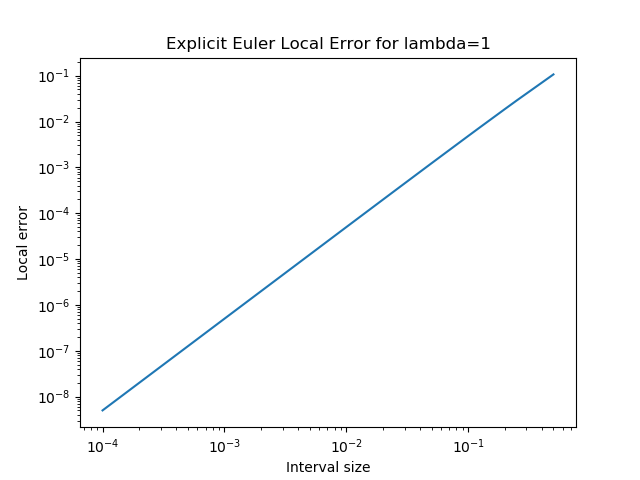
\includegraphics[scale=0.6]{loglog1a1}
		\end{figure}
		We see the local error has a gradient of 2 on the log-log graph.

		\begin{figure}[H]
			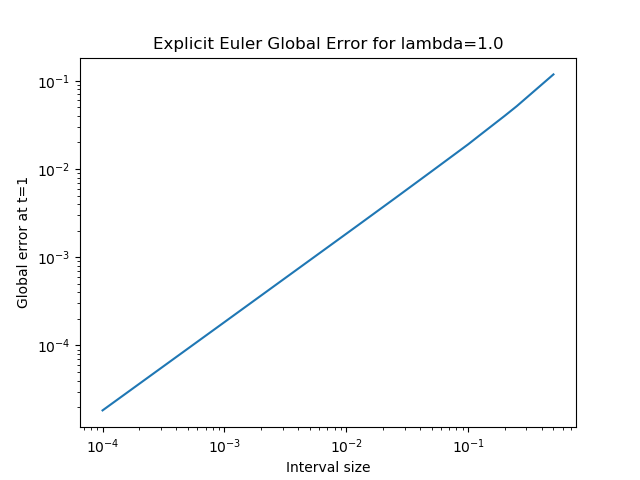
\includegraphics[scale=0.6]{loglog1a1global}
		\end{figure}
		We see the global error has a gradient of 1 on the log-log
		graph, as we would expect for an order 1 method.

		\begin{figure}[H]
			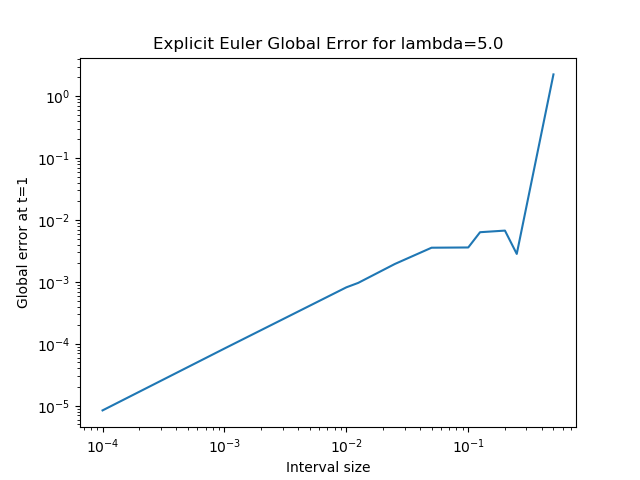
\includegraphics[scale=0.6]{loglog1a5global}
		\end{figure}
		Notice, for $\lambda = 5$, our error leaves the line for
		interval sizes larger than $0.2$, as demonstrated before.

	\item[(b)]
		First, we determine the order analytically. Consider
		\begin{align*}
			x_{j+1} &= \frac{1}{2} (1 + (1 - \lambda h)^2)x_j \\
			&= (1 - \lambda h + \frac{\lambda^2 h^2}{2})x_j \\
			&= (1 - \lambda h + \frac{\lambda^2 h^2}{2})^{j+1} x_0\\
			&= (1 - \lambda h + \frac{\lambda^2 h^2}{2})^{j+1}.
		\end{align*}
		Notice that $1 - \lambda h + \frac{\lambda^2 h^2}{2})^{j+1}$ are
		exactly the first three terms of the tailor series of the
		solution. We calculate the local error for a step-size of $\tau$:
		\begin{align*}
			\epsilon(\tau) &= |e^{- \lambda \tau} - x_{1}| \\
			&= |\sum_{k=3}^{\infty} (-1)^k(\lambda \tau)^k| \\
			&\leq |\tau^3 \sum_{k=3}^{\infty} (-1)^k(\lambda)^k| \\
			&= |\tau^3 (e^{- \lambda} - 1 + \lambda -
			\frac{\lambda^2}{2})| \\
			&\in \mathcal{O}(\tau^3).
		\end{align*}

		The global error at some time $t$ is the calculated as
		\begin{align*}
			\epsilon_{G}(\tau) &= \frac{t}{\tau} \epsilon(\tau)\\
			&\leq \frac{t}{\tau} C |\tau^3| \\
			&=  |t C \tau^2|
		\end{align*}
		which shows that the Heuns method is of order $2$.

		\begin{figure}[H]
			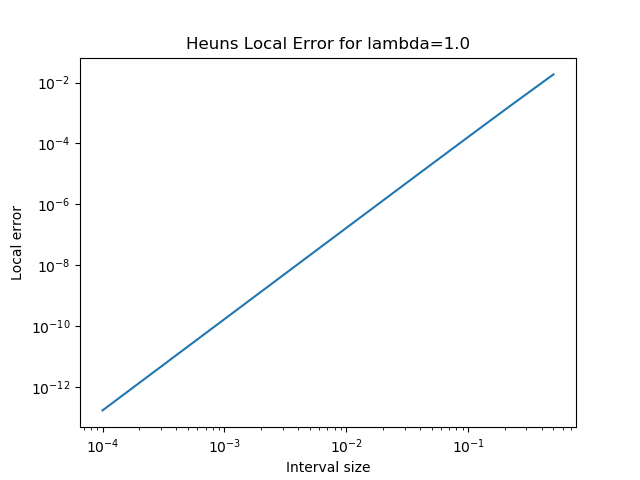
\includegraphics[scale=0.6]{loglog1b1local}
		\end{figure}
		\begin{figure}[H]
			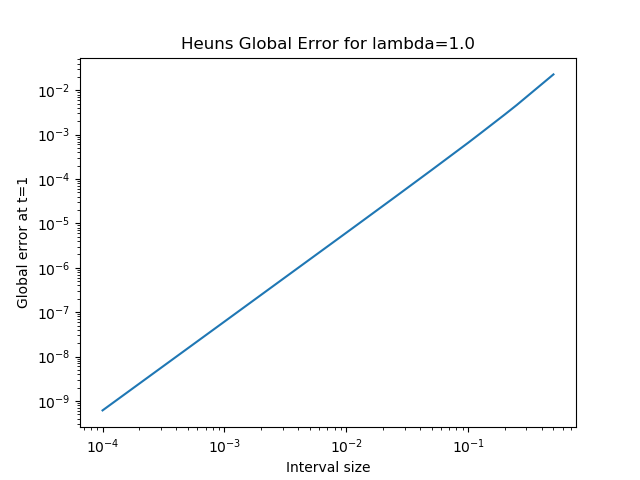
\includegraphics[scale=0.6]{loglog1b1global}
		\end{figure}
		\begin{figure}[H]
			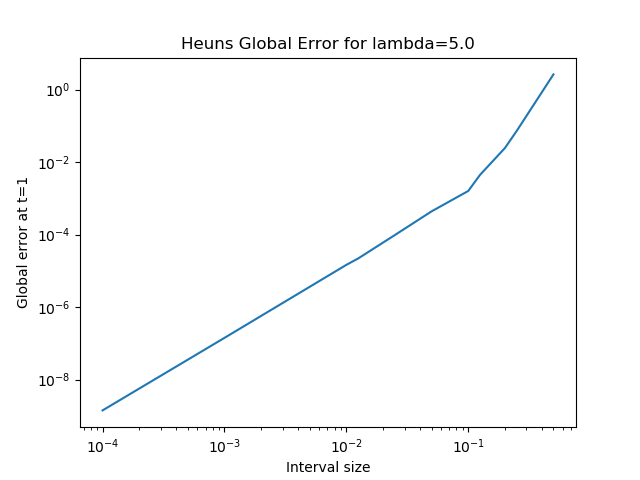
\includegraphics[scale=0.6]{loglog1b5global}
		\end{figure}
		Notice that, while the Heuns method's error also gets worse for
		larger interval values, together with the larger value of
		$\lambda = 5$ it
		only leaves the expected line for
		much larger interval sizes of about $0.1$.
\end{itemize}

\subsection{}
\begin{itemize}
	\item[(a)]
		Notice that if
		\[
			\mathbf{x} =
			\begin{bmatrix}
				x(t) \\
				y(t)
			\end{bmatrix},
		\]
		then
		\begin{align*}
			\mathbf{\dot{x}} &=
			\begin{bmatrix}
				 y(t) \\
				-x(t)
			\end{bmatrix} \\
			&= \begin{bmatrix}
				 0 & 1 \\
				-1 & 0
			\end{bmatrix}
			\begin{bmatrix}
				x(t) \\
				y(t)
			\end{bmatrix}.
		\end{align*}
		So we set
		\[
			A =
			\begin{bmatrix}
				 0 & 1 \\
				-1 & 0
			\end{bmatrix}
		\]
		and the solution to our problem is $\mathbf{x}(t) =
		e^{At}\mathbf{x_0}$.  Notice
		\begin{align*}
			A &=
			\begin{bmatrix}
				 0 &  1 \\
				-1 &  0
			\end{bmatrix} \\
			A^2 &=
			\begin{bmatrix}
				-1 &  0 \\
				 0 & -1
			\end{bmatrix} \\
			A^3 &=
			\begin{bmatrix}
				 0 & -1 \\
				 1 &  0
			\end{bmatrix} \\
			A^4 &= A^0 =
			\begin{bmatrix}
				 1 &  0 \\
				 0 &  1
			\end{bmatrix}.
		\end{align*}
		So
		\begin{align*}
			e^{At} &= \sum_{k = 0}^{\infty}
			(A^{4k} \frac{t^{4k}}{(4k)!} +
			A^{4k+1} \frac{t^{4k+1}}{(4k + 1)!} +
			A^{4k+2} \frac{t^{4k+2}}{(4k + 2)!} +
			A^{4k+3} \frac{t^{4k+3}}{(4k + 3)!}) \\
			&= \sum_{k = 0}^{\infty}
			I \frac{t^{4k}}{(4k)!} +
			A \frac{t^{4k+1}}{(4k + 1)!} +
			A^{2} \frac{t^{4k+2}}{(4k + 2)!} +
			A^{3} \frac{t^{4k+3}}{(4k + 3)!} \\
			&= \begin{bmatrix}
				\sum_{k=0}^{\infty} \frac{t^{4k}}{(4k)!} -
				\frac{t^{4k + 2}}{(4k + 2)!}&
				\sum_{k=0}^{\infty} \frac{t^{4k + 1}}{(4k + 1)!}
				- \frac{t^{4k + 3}}{(4k + 3)!}\\
				\sum_{k=0}^{\infty} \frac{t^{4k + 3}}{(4k +
				3)!}- \frac{t^{4k + 1}}{(4k + 1)!}&
				\sum_{k=0}^{\infty} \frac{t^{4k}}{(4k)!} -
				\frac{t^{4k + 2}}{(4k + 2)!}
			\end{bmatrix} \\
			&= \begin{bmatrix}
				 \cos(t) & \sin(t)\\
				-\sin(t) & \cos(t)
			\end{bmatrix}.
		\end{align*}
		We are given the initial value of
		\[
			\mathbf{x_0} =
			\begin{bmatrix}
				1 \\
				0
			\end{bmatrix},
		\]
		so
		\begin{align*}
			\mathbf{x}(t) &= e^{At} \mathbf{x_0} \\
			&= \begin{bmatrix}
				\cos(t) & \sin(t) \\
				-\sin(t) & \cos(t)
			\end{bmatrix}
			\begin{bmatrix}
				1 \\
				0
			\end{bmatrix} \\
			&= \begin{bmatrix}
				cos(t) \\
				-sin(t)
			\end{bmatrix}.
		\end{align*}

		The stability of the solution can easily determined by simply
		considering a geometric argument.  The matrix we calculated maps
		any point $(x,y)$ to
		\begin{align*}
			(x \cos(t) + y \sin(t),\  &y \cos(t) - x \sin(t)) \\
			&= (x \cos(-t) - y \sin(-t),\  y \cos(-t) + x \sin(-t))
		\end{align*}  This is well known to be the formula for rotating
		the point clockwise around the origin by $t$ radians, which
		preserves distances. In fact
		\begin{align*}
			\left\Vert e^{At} \mathbf{x} \right\Vert
			&= \sqrt{(x \cos(t) + y \sin(t))^2 + (y \cos(t) - x
			\sin(t))^2}
		\end{align*}
		\begin{align*}
			&=  \sqrt{x^2 \cos^2(t) + 2 x y \sin(t) \cos(t) + y^2
			\sin^2(t) + y^2 \cos^2(t) - 2 x y \sin(t) \cos(t) + x^2
			\sin^2(t)} \\
			&= \sqrt{x^2 (\sin^2(t) + \cos^2(t)) + y^2 (\sin^2(t) +
			\cos^2(t))} \\
			&= \sqrt{x^2 + y^2} \\
			&= \left\Vert \mathbf{x} \right\Vert
		\end{align*}

		If
		$\epsilon = \delta > 0$, then for all $\mathbf{x^*} \in
		B_{\delta}(\mathbf{x_0})$, it follows
		\begin{align*}
			\left\Vert e^{At}\mathbf{x_0} -
			e^{At}\mathbf{x^*}\right\Vert
			&= \left\Vert e^{At}( \mathbf{x_0} - \mathbf{x^*})
			\right\Vert \\
			&= \left\Vert \mathbf{x_0} - \mathbf{x^*} \right\Vert \\
			&< \delta \\
			&= \epsilon,
		\end{align*}
		which demonstrates (Ljapunov) stability.  Since the rotation
		operation preserves distances, the solution is decidedly
		not asymptotically stable.
		\begin{figure}[H]
			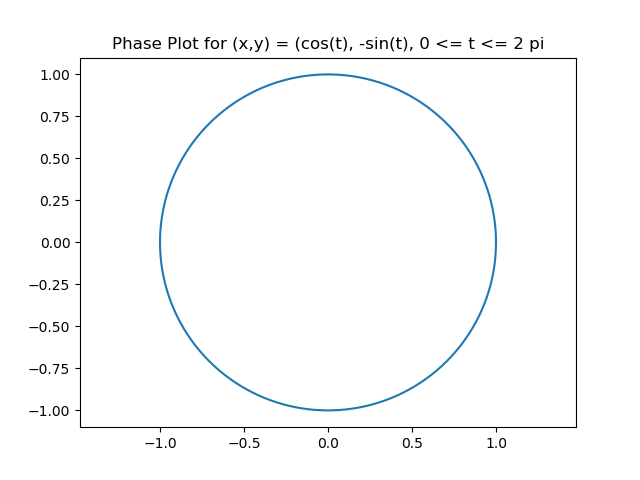
\includegraphics[scale=0.6]{phase_solution2a}
		\end{figure}
	\item[(b)]
		We calculate the step function
		\begin{align*}
			\begin{pmatrix}
				x_{i+1} \\
				y_{i+y}
			\end{pmatrix}
			&=
			\begin{pmatrix}
				x_{i} \\
				y_{i}
			\end{pmatrix}
			+ h f(t_i, 
			\begin{pmatrix}
				x_{i} \\
				y_{i}
			\end{pmatrix}
			) \\
			&=
			\begin{pmatrix}
				x_{i} \\
				y_{i}
			\end{pmatrix}
			+ h
			\begin{pmatrix}
				y_{i} \\
				-x_{i}
			\end{pmatrix} \\
			&=
			\begin{pmatrix}
				x_{i} + h y_{i} \\
				y_{i} - h x_{i}
			\end{pmatrix}.
		\end{align*}
		We use this step function in the explicit Euler method, to
		obtain an approximation, as shown in the following phase graphs.

		\begin{figure}[H]
			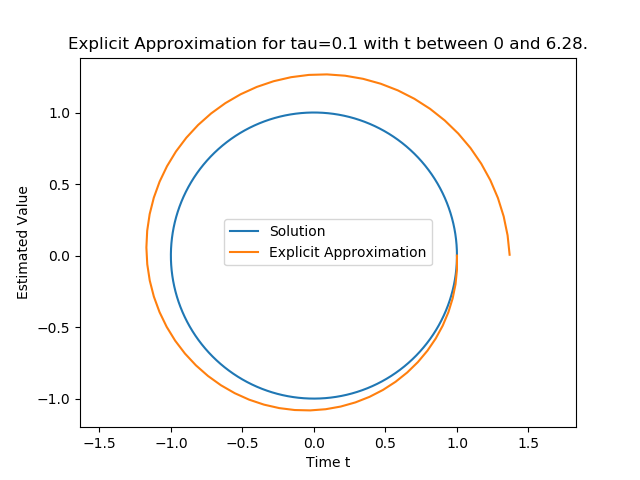
\includegraphics[scale=0.6]{explicitphase2p}
		\end{figure}
		\begin{figure}[H]
			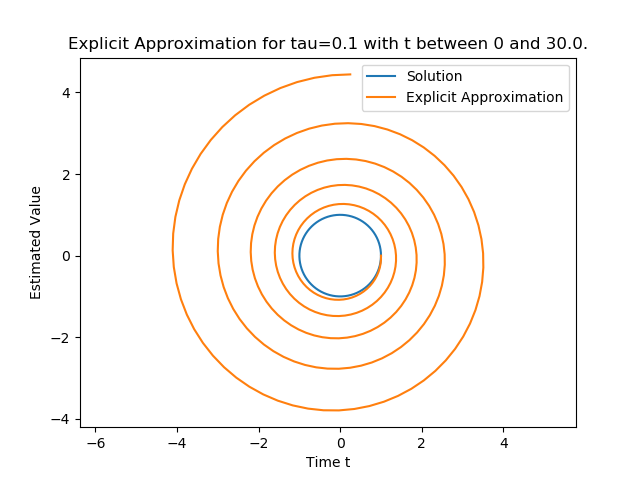
\includegraphics[scale=0.6]{explicitphase30}
		\end{figure}

		To determine stability, consider what happens to the norm in the
		discrete case:
		\begin{align*}
			\sqrt{x_{i+1}^2 + y_{i+1}^2} &= \sqrt{(1 + h^2) x_i^2 + (1
			+ h^2) y_i^2} \\
			&= \sqrt{1 + h^2}\sqrt{x_i^2 + y_i^2}
		\end{align*}
		The difference between discrete
		solution for two different initial values is greater than or
		equal to the differences in the norm
		of the two solutions after a certain number of steps.  At step
		$j$, the difference between the
		norm of two such systems is
		\begin{align*}
			|\mathbf{z_j} - \mathbf{z_j^*} |
			&\geq  ||\mathbf{z_j}| - |\mathbf{z_j^*}|| \\
			&= |(\sqrt{1 + h^2})^j|\mathbf{z_0}| -
			(\sqrt{1 + h^2})^j|\mathbf{z_0^*}|| \\
			&=  (\sqrt{1 + h^2})^j (||\mathbf{z_0}| -
			|\mathbf{z_0^*}||)
		\end{align*}
		Which gets larger as $j$ gets larger.
		So for every$\delta > 0, \epsilon > 0$, for every $\mathbf{z_0^*} \in
		B(\mathbf{z_0})$, there exist a $j > 0$ such that $|\mathbf{z_j}
		- \mathbf{z_j^*} | > \epsilon$. So the solution is not stable. 
	\item[(c)]
		Set
		\[
			\mathbf{z_{i}} =
			\begin{pmatrix}
				x_i \\
				y_j
			\end{pmatrix}.
		\]
		To implement this method, we need a way to calculate
		$\mathbf{z_{j+1}}$ given only $\left\{\mathbf{z_{i}} : 1 \leq i
		\leq j\right\}$. We calculate
		\begin{align*}
			\mathbf{z_{i+1}} &= \mathbf{z_{i}} + hf(t_{i+1},
			\mathbf{z_{i+1}}) \\
			&=
			\begin{pmatrix}
				x_i \\
				y_i
			\end{pmatrix}
			+ h
			\begin{pmatrix}
				y_{i+1} \\
				-x_{i+1}
			\end{pmatrix},
		\end{align*}
		from which we get the linear system of equations
		\begin{align*}
			x_{i+1} &= x_i + h y_{i+1} \\
			y_{i+1} &= y_i - h x_{i+1}.
		\end{align*}
		Solving these for $x_{i+1}$ and $y_{i+1}$, we obtain the explicit
		step
		\begin{align*}
			x_{i+1} &= \frac{1}{1 + h^2}x_i +
			\frac{h}{1+h^2} y_{i} \\
			y_{i+1} &= \frac{1}{1+h^2} y_{i} -  \frac{h}{1+h^2}x_i
		\end{align*}
		which we can use in an algorithm. We draw a phase diagram to see
		its behaviour.

		\begin{figure}[H]
			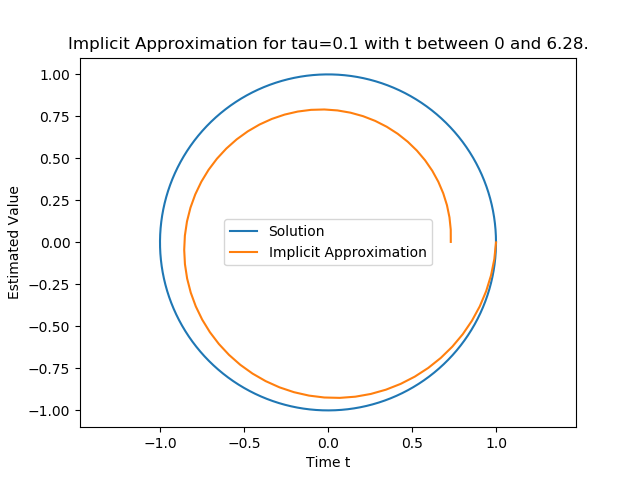
\includegraphics[scale=0.6]{implicitphase2p}
		\end{figure}
		\begin{figure}[H]
			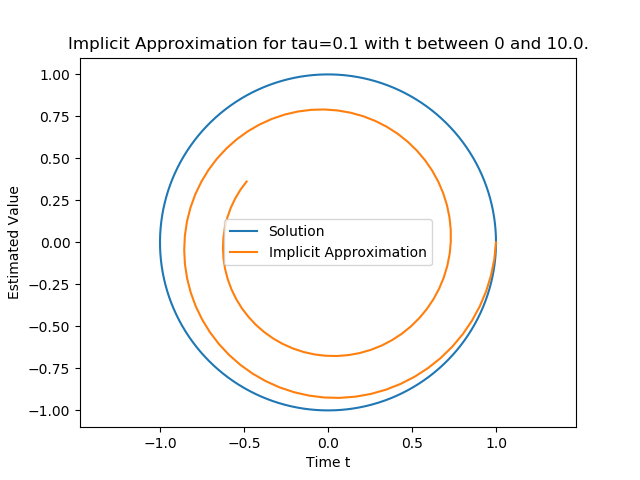
\includegraphics[scale=0.6]{implicitphase10}
		\end{figure}

		As before, we calculate the norm and see that the norm this time
		shrinks:
		\begin{align*}
			|\mathbf{z_i}| &= \frac{1}{(1 + h^2)^2}|\mathbf{z_0}|
		\end{align*}
		This means that the norm approaches zero, so the solution is
		actually asymptotically stable.
\end{itemize}
\end{document}
